\section{Methods}
\label{sec:methods}
{\edits{For a mathematical description of the methods and results, see \citet{Bridgeford2023Jul}. 

Informally, we adopt the following notation to describe batch effect correction. We assume that $Y$ represents an observed measurement of interest (e.g., a connectome), $T$ represents the batch in which the measurement is collected, $X$ represents covariates which are measured associated with the individual for whom the measurement was collected (e.g., age or biological sex), and $Z$ represents covariates which are not measured associated with the individual for whom the measurement was collected. The quantity $Y(t)$ represents the measurement that would have been observed, had the measurement been collected in a given batch $t$. The key distinction is that $Y$ represents the \textit{actual} measurement, which is collected and studied. On the other hand, $Y(t)$ is a hypothetical measurement, which is only actually observed for the case where $T = t$ in most experimental contexts \cite{Cole2009Jan}. That is, individuals have a potential measurement $Y(t)$ for every possible batch, but only a single of these potential measurements are studied under standard observational contexts. That the observed measurements $Y$ given the batch (or measured covariates) and the potential measurements $Y(t)$ do not, in general, have similar distributions is known as the ``fundamental problem of causal inference.'' This problem requires resorting to additional assumptions to make conclusions on the basis of the observed data.

Using this convention, a batch effect is defined in Definition \ref{def:causal_batch_informal}.

\begin{definition}[Causal Batch Effect]
A causal batch effect exists between two batches $t$ and $t'$ if $Y(t)$ and $Y(t')$ have different distributions.
\label{def:causal_batch_informal}
\end{definition}

In light of this definition, a batch effect can be conceptualized as the \textit{potential} measurements having different distributions between a given pair of batches. A batch effect is present if an individual's measurements differ if they \textit{would have been measured} in batches $t$ and $t'$. We can similarly define batch effect correction to be a function of the potential measurements and the batch which remove this disparity, in Definition \ref{def:batch_correct_informal}.

\begin{definition}[Batch Effect Correction]
A function $g$ corrects a batch effect between $Y(t)$ and $Y(t')$ if $g(Y(t), t)$ and $g(Y(t'), t')$ have the same distribution.
\label{def:batch_correct_informal}
\end{definition}

In this case, a function corrects a batch effect if the \textit{potential} measurements have the same distribution after application of the function $g$. Estimation of this function $g$ from the observed data (which, often, does not include realizations of every \textit{potential} measurement for each individual) therefore presents the hurdle of batch effect correction. The major conceptual leap in each of these definitions is that, under standard contexts, these statements are about \textit{potential} measurements rather than \textit{realized} measurements. In other words, causal claims regarding potential outcomes are only valid on the basis of the observed data insofar as the reasonableness of the assumptions upon which they rest.

\subsubsection{Associational Effects}

In an associational context, we observe measurements $y_i$ and batches $t_i$ for each individual $i \in [n]$, so effects can only be determined from $Y$ and $T$. 

\begin{flushleft}\begin{definition}[Associational Effect]
% Suppose the setup described above. 
An associational effect exists between batches $t$ and $t'$ if $Y | T = t$ and $Y | T = t'$ have different distributions.
\label{def:ass_site_effect_informal}
\end{definition}
\end{flushleft}

Similarly, associational effect correction estimates the function $g$ using only the observed measurements and the batches. Under standard contexts, associational effects will often poorly characterize whether a batch effect is present. Consider, for instance, if in one batch $t$, we tend to measure older individuals, whereas in another batch $t'$, we tend to measure younger individuals. If age is related to the measurement we obtained, then the differences between $Y | T = t$ and $Y | T = t'$ could be due to age or batch identity, and we have no way of differentiating whether the effect is a \textit{bona fide} batch effect versus merely an associational effect. A sufficient condition for an associational effect to facilitate detecting or estimating a batch effect would be that individuals are randomized to each batch, in that individuals are assigned to be measured in particular batches \textit{pre-hoc}. Associational effect detection can be facilitated via \Dcorr~\cite{Szekely2007Dec} and associational effect correction can be facilitated via \Combat~\cite{Johnson2007Jan}.

\subsubsection{Conditional Effects}

In a conditional context, we observe measurements $y_i$, batches $t_i$, and covariates $x_i$ for all individuals $i \in [n]$, so effects can be determined from $Y$, $T$, and $X$.

\begin{flushleft}\begin{definition}[Conditional Effect]
A conditional effect exists between batches $t$ and $t'$ if for some covariate $x$, $Y | T = t, X = x$ and $Y | T = t', X = x$ have different distributions.
\label{def:ass_site_effect_informal}
\end{definition}
\end{flushleft}

Conditional effect correction estimates the function $g$ using the observed measurements, the batches, and the covariates. Conceptually, a conditional effect is equivalent to a batch effect if two conditions hold:
\begin{enumerate}[leftmargin=*]
    \item  the measured covariates overlap in distribution between the batches (propensity overlap), and
    \item given the measured covariates, we can ignore how people ended up in one batch versus the other.
\end{enumerate}

The former condition denotes that both batches must contain similar groups of people (in terms of measured covariates), and the latter condition specifies that the measured covariates $X$ tell us all of the information needed to ``exchange'' measurements from one batch to the other. Borrowing the preceding example, even if we observe more young people in a batch $t$, that we still observe \textit{some} young people in the other batch $t'$. In this sense, the measured covariates contain the information needed to ``deconfound'' disparities that might be batch effects or veridical effects due to upstream covariates. Therefore, when we make subsequent comparisons, we do not need to guess what people with similar covariates would have looked like in the other batch, and vice versa.

In this fashion, our comparisons can be thought of as locally (with respect to the covariates) exchanging a realized measurement $Y$ in batch $t$ with a realized measurement $Y$ in batch $t'$, where both individuals have similar covariates $x$. Intuitively, these comparisons can therefore be conceptualized as synthetically comparing $Y(t)$ and $Y(t')$ (the target estimand for establishing a batch effect) by using observed measurements $Y$ from individuals who are similar on the basis of the covariates $X$ between the two batches. The former condition ensures that we can make this intuitive step over the entire span of covariates in our batches. Conditional effect detection can be facilitated via \cdcorr~\cite{Wang2015}, and conditional effect correction can be facilitated via \ccombat~\cite{Johnson2007Jan}.

In practice, we never know whether the propensity distributions overlap; we can only estimate them from the data. If our estimated propensities do not overlap given finite data, we again cannot reasonably differentiate between differences in the two groups being due to \textit{bona fide} batch effects or empirical differences in the propensity distributions. This motivates a third approach. 

\subsubsection{Adjusted Effects}

As before, we observe measurements $y_i$, batches $t_i$, and covariates $x_i$ for all individuals $i \in [n]$, and we determine effects from $Y$, $T$, and $X$. Prior to assessing the equality of any distributions, however, we weight the observations such that the observed covariate distributions are rendered approximately overlapping.

\begin{flushleft}\begin{definition}[Adjusted Effect]
An adjusted effect exists between batches $t$ and $t'$ if after re-weighting samples such that $X | T = t$ and $X | T = t'$ are approximately overlapping (or, alternatively, approximately equal), $Y | T = t, X = x$ and $Y | T = t', X = x$ have different distributions.
\label{def:ass_site_effect_informal}
\end{definition}
\end{flushleft}

Adjusted effect correction amounts to estimating the function $g$ using the observed measurements, the batches, and the covariates, but placing higher priority on up-weighted samples and lower priority on down-weighted samples in the estimation process depending on whether they are sufficiently represented in both batches of interest. Adjusted effects, by default, satisfy the first criterion for a conditional effect to be a batch effect. This is because rendering measured covariate distributions approximately equal intuitively is a more strict criterion than simply ensuring that they approximately overlap. The reason that we believe that re-weighting to ensure approximate covariate distribution equality is desirable for effect correction, versus simply approximate covariate overlap, is discussed in Section \ref{sec:results:sims} and Appendix \ref{app:sim_batch_adj}. Adjusted effect detection can be facilitated via \ccdcorr~\cite{Bridgeford2023Jul}, and adjusted effect correction can be facilitated with \cccombat~(described in Section \ref{sec:cccombat}).

We still must satisfy the latter criterion for a conditional effect to be a batch effect; that is, given the measured covariates, we can ignore how people ended up in one batch versus the other. This assumption has the same interpretation as before.

\subsubsection{Crossover Effects}

We observe measurements $y_i(t)$ and covariates $x_i(t)$, for all individuals $i \in [n]$ and for all batches $t \in [T]$. In this case, we can make statements on the basis of $Y(t)$, and may not need to resort to local exchangeability (similar individuals across batches) as before. \textit{Crossover effects in general require the fewest assumptions to derive causal conclusions, since we directly observe all possible potential measurements for each individual}.

\begin{flushleft}\begin{definition}[Crossover Effect]
A crossover effect exists between batches $t$ and $t'$ if, given that $\left(X(t), Z(t)\right)$ and $\left(X(t'), Z(t')\right)$ are sufficiently similar, $Y(t)$ and $Y(t')$ have the same distribution.
\label{def:ass_site_effect_informal}
\end{definition}
\end{flushleft}

We are certain that any \textit{traits} of the participants (i.e., variables that are constant for a given participant, such as genome) are the same across the two groups since the group members are identical (even if we did not measure these traits). However, \textit{states} may differ as they may be functions of location or time. For example, if being measured impacts subsequent states, then a crossover effect may not be indicative of a causal batch effect without further assumptions and/or experimental design considerations (such as randomizing exposure order across participants, or resorting to adjusted effect strategies as before if these states are measured). 

In the case where participant states are unchanging or are randomized, we can resort directly to associational strategies for subsequent detection or removal, and can make causal conclusions about batch effects with few additional considerations. In the case where participant states are changing and are not randomized but are measured, we can resort to adjusted strategies for adjusted effect detection or removal. For the latter, we need to make the same assumptions as before; that is, that given the measured covariates (which include the changing states), we can ignore how people ended up in one batch versus the other.}}

\subsection{Detecting and mitigating causal batch effects}
\label{sec:cccombat}
At present, literature approaches for detecting and mitigating batch effects tend to focus attention heavily on effects which could be classified as associational or conditional, which for the above listed reasons, fail to adequately account for confounding biases. To this end, we propose a simple technique to augment associational and conditional strategies and derive stronger causal claims. We propose the following strategy:
\begin{enumerate}[leftmargin=*]
    \item Use classical causal procedures to re-weight the measurements from the batches so that the demographic distributions across all batches to be considered overlapping or are approximately equal. For rendering the covariate distributions approximately overlapping, we leverage vector matching \cite{Lopez2014}. For rendering the covariate distributions approximately equal, we leverage propensity trimming followed by nearest neighbor matching \cite{Stuart2010Feb,Powell2020Sep}. 
    \item Apply classical procedures for detection or removal of {\edits{conditional}} effects. For the purposes of elucidating the benefits of this perspective, we choose to apply our techniques to \cDcorr~for batch effect detection \cite{Wang2015,Bridgeford2023Jul}, and \ccombat~for batch effect removal \cite{Pearl2010Jul,Johnson2007Jan,Leek2010-ua,Leek2015-jc,Wachinger2020Feb,Yu2018Nov,Pomponio2020Mar}.
\end{enumerate}

For a more technical description of the causal procedures employed in this manuscript, see Appendix \ref{app:causal_procedures}. It is important to note that we do \textit{not} make the claim that the specific choices for re-weighting measurements (propensity trimming followed by nearest-neighbor matching) are necessarily the best possible approach to balancing the demographic distributions across the batches. Indeed, there are almost two decades of research dedicated towards making these design choices for observational studies. Rather, we chose simple, principled, and straightforward approaches for illustrative purposes. Our simulations contained herein and in our related manuscript \cite{Bridgeford2023Jul} elucidate that even these possibly simplistic balancing approaches are sufficient to highlight substantial shortcomings in the existing literature for batch effects and causal effect testing, as well as the substantial benefits of a causal perspective.

\subsection{Batch effects in biological datasets}

\begin{figure}[h]
    \centering 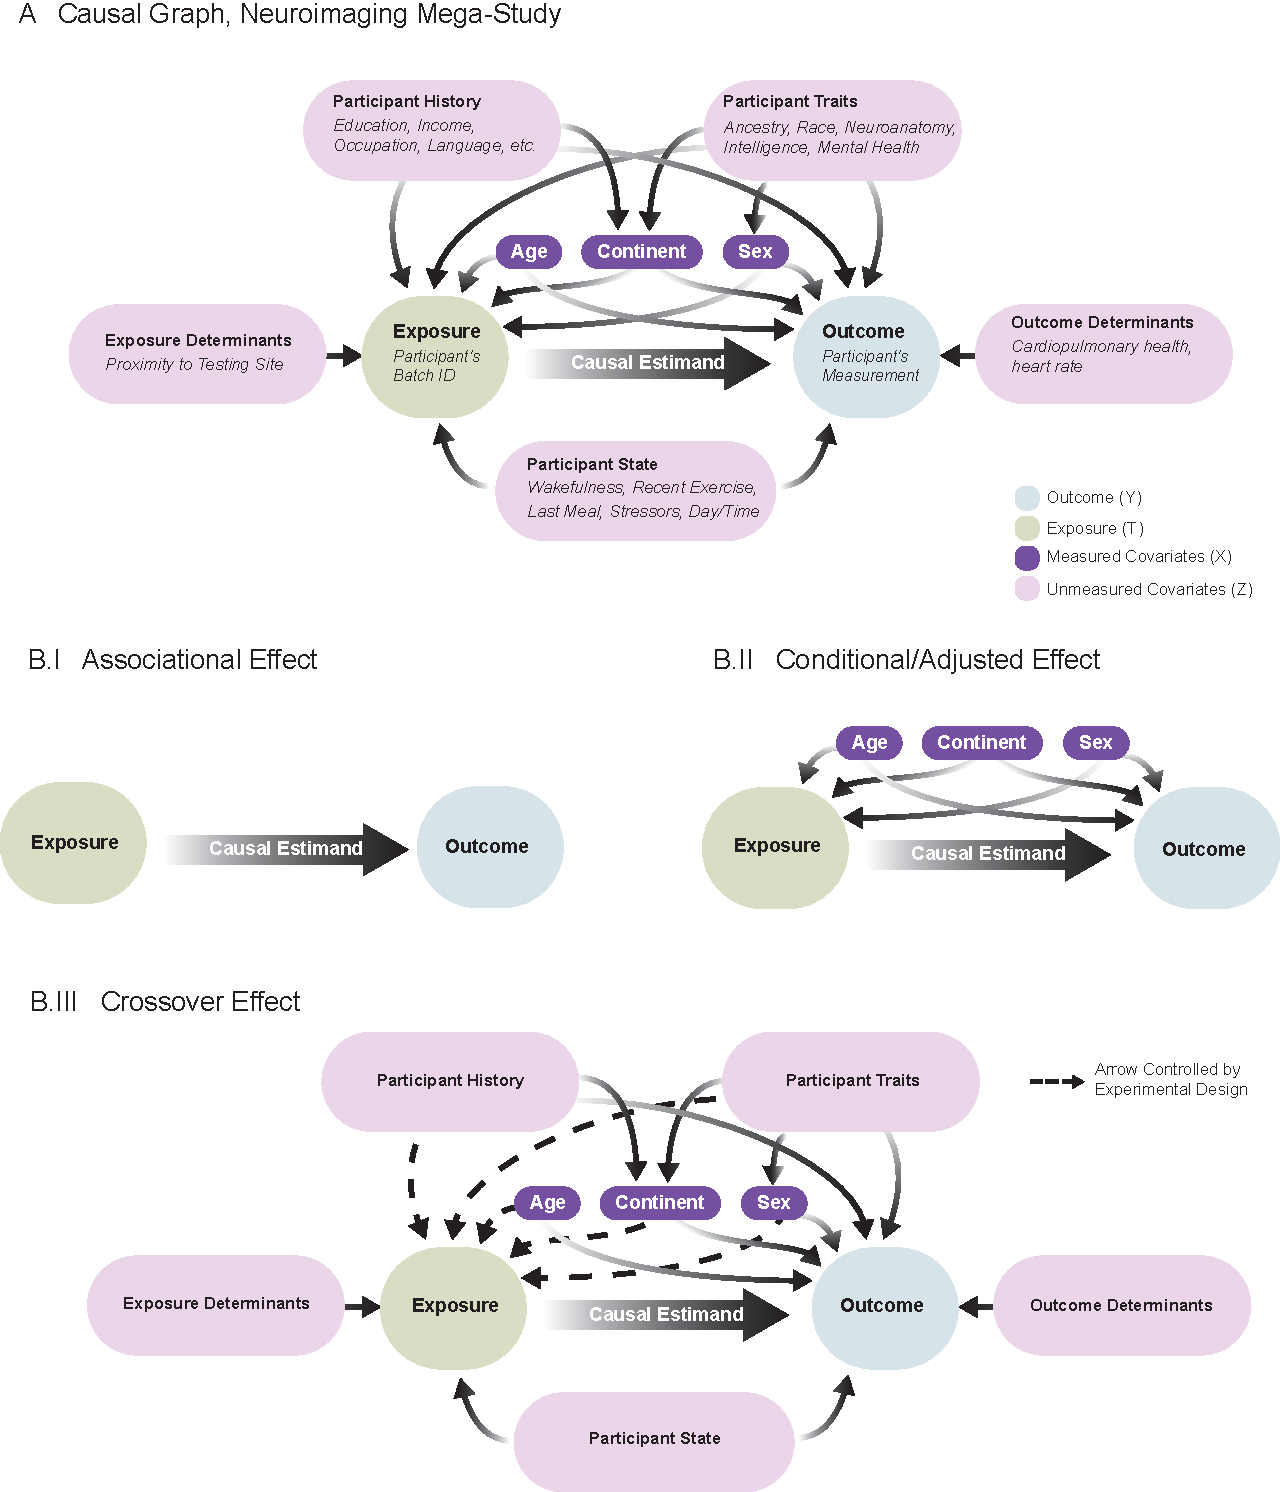
\includegraphics[width=\linewidth]{Figures/Content/CoRR_dag.pdf}
    \caption{\textbf{Causal Graph of Study Covariates}. \textbf{(A)} A causal directed acyclic graph (DAG) illustrating potential relationships which can reasonably be assumed to underlie a mega-study. Descriptions reflect possible attributes that might fall into the specific exposures, outcomes, and covariates for a neuroimaging study, for illustration purposes. \textbf{(B)} DAGs which illustrate the assumptions which underlie assorted effects in order for those effects to be causal. Associational effects \textbf{(B.I)} are causal when all external covariates are independent the exposure and outcome. Conditional effects and adjusted effects \textbf{(B.II)} are causal when the strong ignorability condition holds, and in particular when the measured covariates close backdoor paths. Crossover Effects \textbf{(B.III)} are causal when participant states are non-confounding between the exposure and the outcome. The experimental design of a crossover study ensures that other forms of measured and unmeasured covariates are non-confounding.}
    \label{fig:dag}
\end{figure}
The four effects discussed above have immediate practical implications on measuring batch effects in modern biological datasets. To this end, we demonstrate the applicability of these effect types in the context of a neuroimaging mega-study, in which measurements are collected from individuals across various batches (the \textit{exposures}). The logical process, however, extends beyond this context to many other biological data modalities, such as genomics. Figure \ref{fig:dag}A shows a directed acyclic graph, or DAG, which underlies a typical mega-study. The exposure is the batch in which participants' data are collected, and the outcomes are the measurements themselves. We seek to estimate the \textit{causal estimand}, which is the causal effect of the exposure to a particular batch on the outcome (the \textit{measurement}). Numerous covariates, both known and unknown, impart potentially confounding biases, in which the variables can influence both the exposure and the outcome.
For instance, one batch collected in a children's hospital may tend to over-sample younger individuals relative to other batches, and younger children may have distinct patterns of brain connectivity compared to older children. {\edits{For this investigation, we use age and sex (which are commonly used for adjusting for batch effects) as well as continent as measured covariates in subsequent analyses. We depart from many previous harmonized analyses by leveraging continent due to the growing literature \cite{JianqiaoGe2023Jan,Park2010Jul} which suggest differences in brain function for individuals across cultures. Unaccounted confounding via culture/race (for which continent serves an imperfect surrogate) may yield confounding biases in subsequent analysis, in which batch effects may be conflated with veridical demographic differences.}} Unmeasured covariates are often prominent confounders in biological datasets, making proper causal analyses troublesome. \textit{Participant history} involves variables related to specific life experiences, both environmental and societal, that the individual has been exposed to. \textit{Participant traits} are characteristics of a person that remain relatively constant over time. \textit{Participant states} refer to characteristics of a person that change over an individual's lifetime. \textit{Exposure determinants} are factors which impact batch membership for a particular individual, but do not impact the measurement itself. \textit{Outcome determinants} are factors which do not impact the batch assignment, but impact the outcome.

Figure \ref{fig:dag}B illustrates the implicit DAGs that are sufficient such that if they characterized the data, then each of the four effect types discussed above become valid causal batch effect estimands. 
If no covariates exist (observed or unobserved), then an associational effect is a causal effect (Figure \ref{fig:dag}B.I). 
% TODO re-read below
% While conditional and associational effects can be causal in the presence of confounding when confounding variables are measured, neither effect is causal when confounding variables are unmeasured (Figure \ref{fig:dag}B.II).
Crossover effects can account for many types of measured and unmeasured covariates which are confounding (Figure \ref{fig:dag}B.III). Because of the crossover property, the batches will be balanced across certain measured and unmeasured covariates, specifically patient history and traits. Hence, many of the confounding variables from Figure \ref{fig:dag}A are deconfounded. However, unmeasured changes in participant state between different exposure groups (such as measuring individuals only during the daytime in one batch and only during the night time in another batch) remain potential confounders if not carefully balanced across exposure groups through either randomization or direct experimental intervention. 

\section{Results}
\label{sec:results}
\subsection{Traditional approaches fail to adequately remove batch effects when covariate overlap is poor}
\label{sec:results:sims}
We constructed simulations to help us understand the differences between associational or conditional reasoning and causal reasoning. Figure \ref{fig:sim_nlin_adjust}(A).I. shows a simulation where the outcome of interest (e.g., a feature of a connectome, $y$-axis) is associated with a covariate of interest ($x$-axis) through a non-linear relationship (the sigmoid). If samples are from the blue batch, they are offset $1$-unit higher than samples from the orange batch. $N=500$ samples are drawn with equal probability from each batch. In the high overlap regime, the orange and blue batches have the same covariate distribution. Figure \ref{fig:sim_nlin_adjust}(B).I. shows the expected signal (solid line) for each batch, along with the difference between the expected signal for each batch (gray box). These curves are shown along with the group-specific linear model fit (dashed lines) estimated from the sample points, which is the model that is later used by \ccombat~for batch effect adjustment. Figure \ref{fig:sim_nlin_adjust}(C).I. and Figure \ref{fig:sim_nlin_adjust}(D).I. show the impact that \ccombat~and \cccombat~have on the expected signal at a given covariate level. Intuitively, one would anticipate that a batch effect correction strategy should place the expected signals virtually overlapping after correction, since the batch effect is characterized by the expected signals in each group differing by an offset factor. For both strategies, the expected signal after correction is virtually the same for each of the two batches, indicating that the batch effect has been successfully removed. \edits{We compute the mean average absolute difference (AAD) across included covariate values of the two lines over $R=1$,$000$ trials, where a mean AAD of $1$ corresponds to the residual disparity on average equaling the original batch effect, and a mean AAD of $0$ corresponds to no residual disparity. The mean AAD is discussed in Appendix \ref{app:maad}. We find that \ccombat~has a mean AAD of $.058$, and \cccombat~a  mean AAD of $.047$, with \cccombat~having a lower mean AAD about $62\%$ of the time.}

Figure \ref{fig:sim_nlin_adjust}(A).II. shows similar plots; however, the covariate distributions have been shifted such that they no longer overlap perfectly. The orange batch has a left-shifted covariate distribution, and the blue batch has a right-shifted covariate distribution (the covariate is \textit{confounding} the relationship between the outcome and the batch). Figure \ref{fig:sim_nlin_adjust}(B).II. shows that while the expected signal in each batch at a given covariate level is the same as in Figure \ref{fig:sim_nlin_adjust}(B).II., the linear model fits for each group estimated from the sample now differ (the lines are rotated slightly in a clockwise direction, and are now offset further apart). Figure \ref{fig:sim_nlin_adjust}(C).II. shows that after correction, the expected signal at each covariate level do not overlap; in fact, they differ more after correction than before. This is because the model being employed by \ccombat~is biased under the given true data distribution. Figure \ref{fig:sim_nlin_adjust}(D).II. shows that, unlike \ccombat, \cccombat~restricts inference to the region of shared covariate overlap between the two batches, and does not perform inference that is unsupported by the data. This is indicated by the fact that the expected signal after correction has been restricted to no longer include the left-most and right-most portions of the covariates. Within this region, the expected signal for each batch after correction are much closer, indicating that the batch effect has been nearly entirely removed after \cccombat. \edits{Over all trials, we find that \ccombat~has a mean AAD of $1.04$, and \cccombat~a mean AAD of $0.22$, with \cccombat~always having a lower mean AAD.}

Figure \ref{fig:sim_nlin_adjust}(A).III. has furthered this trend such that there are almost no samples in a region of shared covariate overlap between the two batches. In Figure \ref{fig:sim_nlin_adjust}(B).III. the expected signal in each batch at a given covariate level is the same as in Figure \ref{fig:sim_nlin_adjust}(B).I., but the per-group linear model fits are now even further offset. \edits{This has the effect that in Figure \ref{fig:sim_nlin_adjust}(C).III., the expected signal after correction has a mean AAD of $3.03$, exceeding the original batch effect by over $200\%$.} On the other hand, \ref{fig:sim_nlin_adjust}(D).III. shows that \cccombat~would indicate to not perform inference at all on the batches due to the fact that there are no portions of the covariate range in which the two batches have samples which could be compared. \edits{\cccombat~only executes on $26$ of the trials, and has a mean AAD of $0.369$, always lower than that of \ccombat~for trials in which it could be executed.}

\begin{figure}[h]
    \centering
    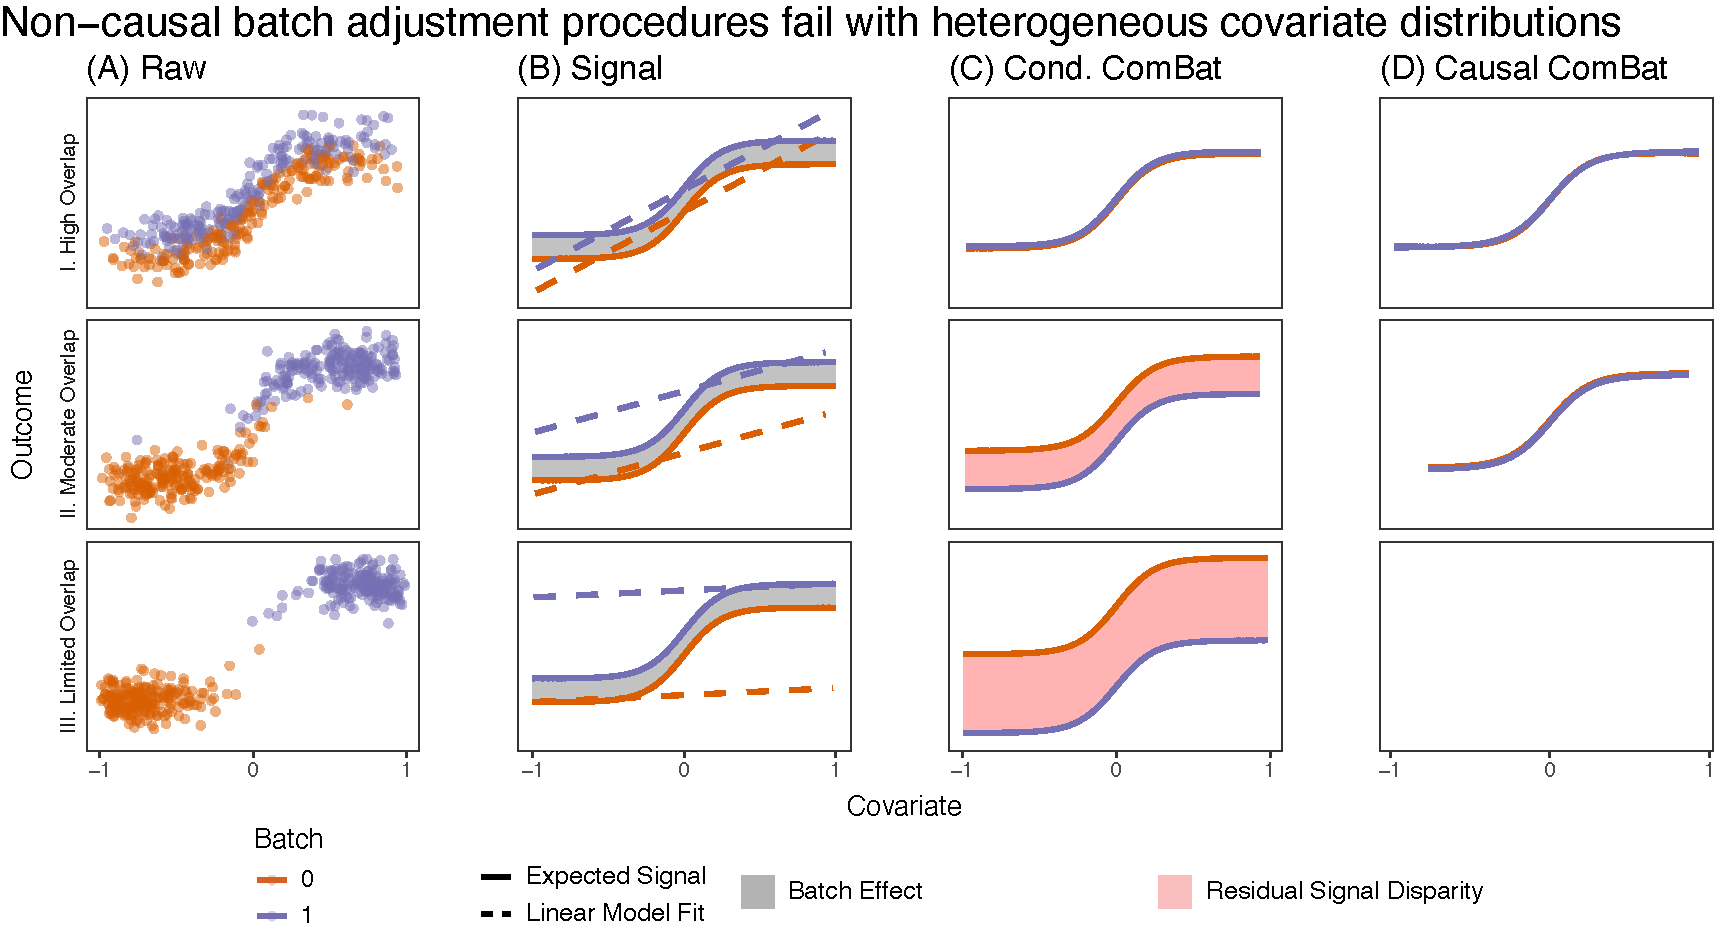
\includegraphics[width=\linewidth]{Figures/Content/sim_nlin_adjust.pdf}
    \caption{\textbf{Non-causal procedures are subject to strong biases without covariate matching}. $N=400$ points are simulated from either batch $0$ or batch $1$ in (A). In (B), the expected signal at a given covariate level is indicated by the solid lines. The batch effect is the difference between the two solid lines (gray box). The estimated linear model fit employed by \ccombat~is indicated with the dashed line. After adjustment (C. and D.), the original expected signal relationship is passed through the trained model, and any residual difference between the true signals of the two batches is termed a residual signal disparity (red box). When coverlap overlap is high in I, both \ccombat~and \cccombat~remove the batch effect successfully, and the expected signal after correction accurately overlaps. With moderate covariate overlap in II, the limitations of the \ccombat~model introduce residual bias that results in an over-correction of the batch effect (on average, the residual signal difference is about about equal to the original batch effect). While \cccombat~reduces the covariate space for inference to remove samples with covariates unlike the other batch (the covariate region to the far left and far right), the samples within the region of covariate overlap are in general reasonably corrected for a batch effect without corrupting the covariate/outcome signal relationship (on average, the residual signal difference is about $20\%$ the original batch effect). When covariate overlap is low in III, Causal strategies tend to report that no inference can be performed, which in our opinion, is the correct procedure. On the other hand, conditional strategies may impart substantial residual signal disparities (on average, about $300\%$ the scale of the original batch effect).}
    \label{fig:sim_nlin_adjust}
\end{figure}

In Appendix \ref{app:sim_effect} and Appendix \ref{app:sim_batch_adj}, we explore further implications of using causal techniques for batch effect detection and removal (and more broadly, causal effects in general) respectively across both linear and non-monotonic regimes to supplement the non-linear regime investigated here. Conceptually, researchers may feel as though they are left with a tradeoff:
\begin{enumerate}[leftmargin=*]
    \item When datasets do not have high overlap demographically, the (implied or explicit) limitations of a model leveraged by a batch effect detection or correction technique can impart substantial bias on the conclusions of the investigation. While the limitations or shortcomings may \textit{seem} inconsequential, the scale of the residual signal disparities imparted can dwarf the original batch effect, and yield measurements which are \textit{more} dissimilar than prior to batch effect adjustment, as we saw in Figure \ref{fig:sim_nlin_adjust}(C).II. and (C).III.
    \item Enforcing demographic overlap mechanistically through propensity trimming and/or matching may \textit{seem} like it yields fewer samples for analysis, or narrows the scope of conclusions.
\end{enumerate}
In practice, the reality is that with biological data, there are \textit{no} ground truths. As a result, there is no way to evaluate the introduction of imparted residual bias, and no way to know whether downstream conclusions are a product of imparted residual biases. This means that any statistical inference we derive may be arbitrarily true or false, and we have no way of qualifying in which pool our inference stands. 

When we mechanistically re-weight the data to impose demographic overlap, proper statistical inference tempers conclusions as a direct consequence of the smaller demographic region under consideration. Stated another way, this means that when we balance \textit{prior to} detecting or correcting for batch effects, we have tools which allow us to make internally valid conclusions supported by the data in regions in which the data \textit{are able}. This means that, although our conclusions may not apply to the \textit{entire} region of covariate support in the observed data (such as, in Figure \ref{fig:sim_nlin_adjust}(D).II., where we were only able to perform analysis in the region of shared support), they will be \textit{statistically and methodologically valid} with respect to the re-weighted population that we \textit{did} analyze.

\subsection{The CoRR Studies have disparate demographic characteristics}
\label{sec:demo}
% refer back to description of CoRR in non-novel methods
Figure \ref{fig:demographic}A  explores the demographic characteristics for the individuals in the CoRR mega-study. Many of the studies have a narrow age range, and several studies only include females. Because sex \cite{Weis2020Mar,Ingalhalikar2014Jan,Satterthwaite2015Sep}, age \cite{Varangis2019,Sala-Llonch2015,Hampson2012Sep}, and continent \cite{Misiura2020} are variables that have been associated with brain connectivity, they serve as conditional covariates used in our investigation.

\begin{figure}[h]
    \centering
    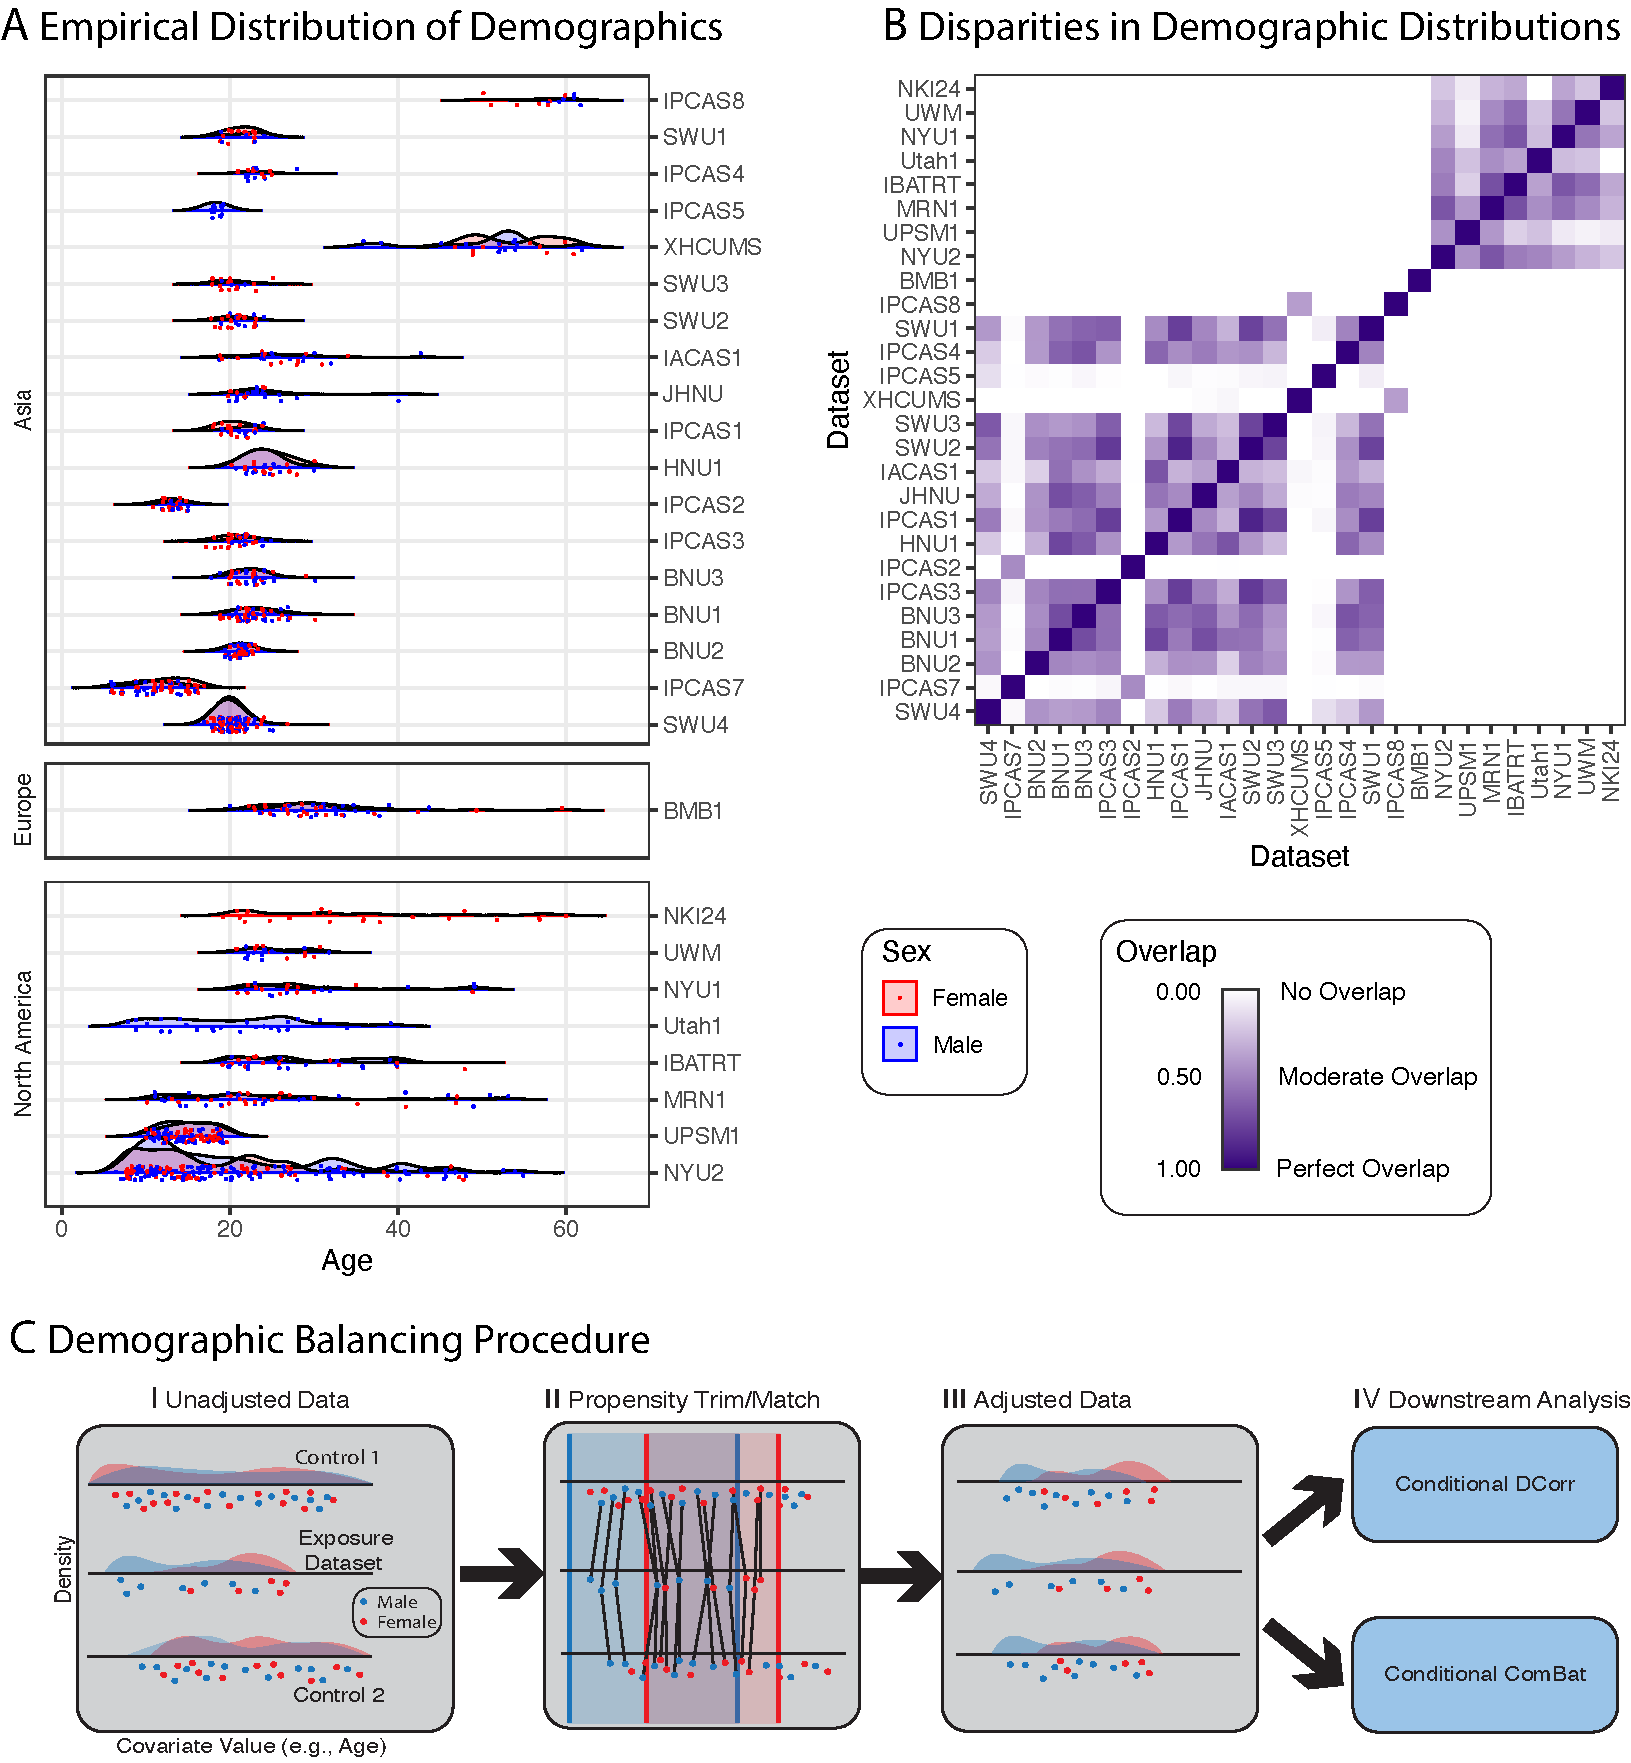
\includegraphics[width=\linewidth]{Figures/Content/demographic.pdf}
    \caption{\textbf{Demographic data for each of the $N=27$ studies from the CoRR Mega-Study}. \textbf{(A)}  Each point represents the age of a participant corresponding to a single measurement, rows are studies, boxes are continents, and color indicates sex. 
    % Empirical density is estimated across individuals corresponding to each sex within each study, where height is scaled by the number of measurements for each $(\textrm{sex}, \textrm{study})$ pair. 
    \textcolor{black}{\textbf{(B)} Even with only $3$ covariates made available (sex, age, continent of measurement) the CoRR studies generally show extremely poor covariate overlap \cite{Pastore2019}. This makes inference regarding batch effects difficult. \textbf{(C)} The demographic balancing procedure, to demographically align poorly balanced datasets using Causal \Dcorr~or \cccombat. (C.I) The unadjusted datasets are imbalanced in covariate distributions. The smallest dataset, the \textit{reference}, has a narrower age distribution than the controls. (C.II) Propensity trimming (shaded boxes) and matching (lines) are conducted to identify reasonable matches between the reference and the control datasets. (C.III) The adjusted datasets have far improved demographic overlap after propensity trimming, matching, and removing reference subjects who do not have suitable matches in the control datasets. (C.IV) Downstream batch effect detection via \Dcorr~or correction using \Combat~are performed on the data using conditional strategies on the adjusted data.}}
    \label{fig:demographic}
\end{figure}

\textcolor{black}{Figure \ref{fig:demographic}B investigates the level of demographic overlap in the CoRR mega-study, using the distribution-free overlapping index \cite{Pastore2019}, as discussed in Appendix \ref{app:overlap}. Many of the datasets do not overlap at all, and inference on the presence or absence of batch effects would be entirely model-based, as-per Figure \ref{fig:sim_nlin_adjust}.III. Further, while some of the datasets overlap, the level of balance varies widely. In the case where demographic imbalances are substantial, the detection or removal of batch effects would be extremely subject to model-based assumptions, as-per Figure \ref{fig:sim_nlin_adjust}II. From a causal perspective, this is troublesome, as the covariate records for the CoRR mega-study only include three covariates: age, sex, and continent of measurement. The addition of successive covariates can only reduce the estimated overlap between the pairs of datasets, so having poor overlap on such a coarse set of covariates indicates that the actual demographic overlap may be even lower. This would be problematic if, for instance, unmeasured covariates (such as participant mental health) are confounders.}

\subsection{Detecting Batch Effects in the CoRR mega-study}

\begin{figure}[h]
    \centering
    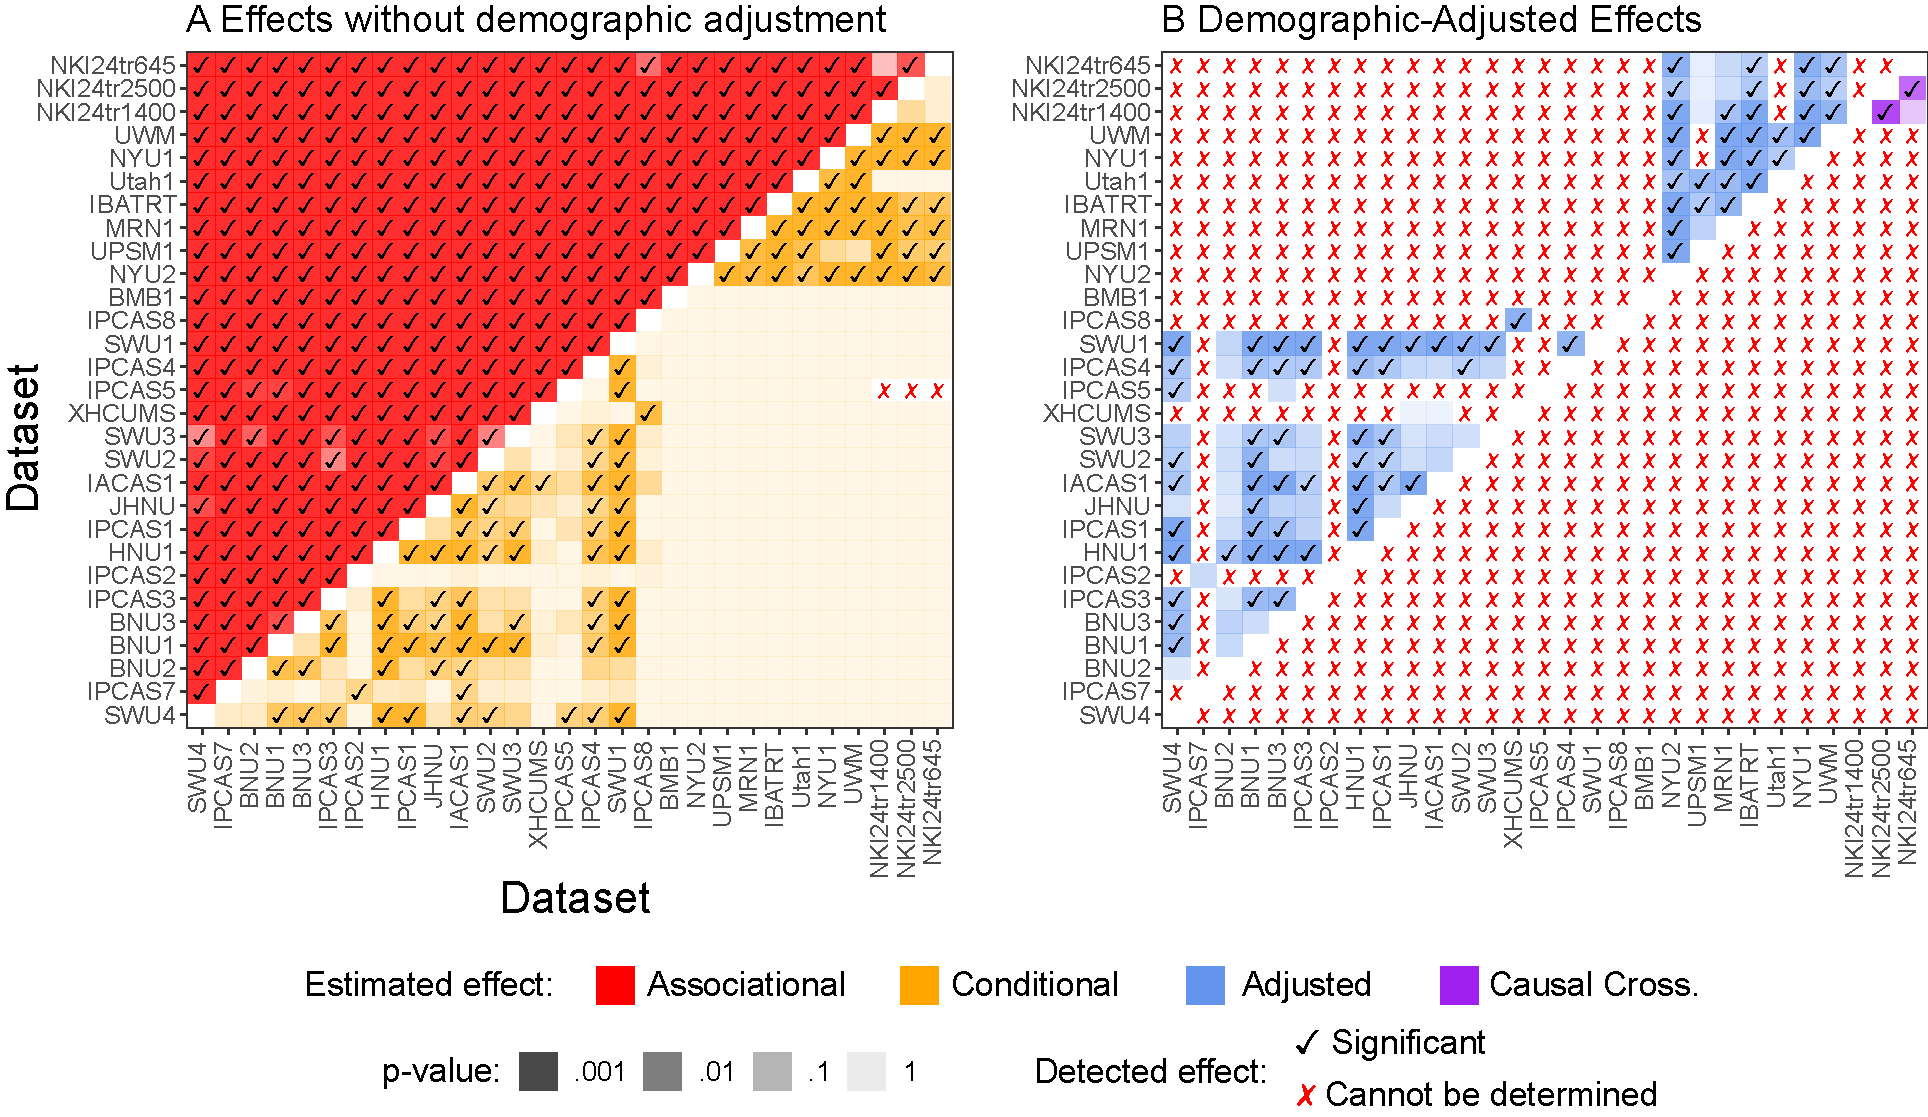
\includegraphics[width=\linewidth]{Figures/Content/raw_pairwise.pdf}
    \caption{\textbf{Comparison of Estimated Effects for CoRR Mega-Study}. Heatmaps indicating the $p$-value of effect estimates per pair of studies. Studies are organized by continent, followed by the number of samples in the study. Comparisons which are significant at $\alpha=.05$ are indicated by a black check. Since effects are symmetric (an effect between batch $t$ and $t'$ is equivalent to an effect between batch $t'$ and $t$), we collapse symmetric heatmaps into a single triangle for each effect type. \textbf{(A)} Effects which can be estimated but do not make direct adjustments for demographics. Associational and conditional effects can almost always be estimated between pairs of studies, so long as they share overlap in at least one covariate (IPCAS5 and NKI24 studies are entirely male or entirely female, entirely different continents, and entirely different age distributions, respectively, red Xs). \textbf{(B)} Effects which adjust for demographics through covariate adjustment. Squares in which an effect was not estimable due to covariate misalignment are indicated by a red X. Effects which adjust for demographics require covariate overlap across all covariates, which is indicated in Figure \ref{fig:demographic}B. A direct comparison of Figure \ref{fig:demographic}B between the conditional and adjusted procedures reveal that whereas conditional procedures tend to ``fail to reject'' with low or zero covariate overlap, adjusted procedures tend to avoid inference entirely.
    }
    \label{fig:raw_pairwise}
\end{figure}

Figure \ref{fig:raw_pairwise}A explores the four effects defined above in fMRI connectomes from the CoRR mega-study. {\edits{The majority of associational effects (99.8$\%$) are significant (distance correlation two-sample test, BH correction, $\alpha=0.05$). When we account for demographic covariates using conditional approaches, this drops to 25.8\% (conditional distance correlation two-sample test, BH correction, $\alpha=0.05$). Conceptually, both of these approaches are overly simplistic for concluding that a causal batch effect is indeed present because they fail to account for non-overlap of the covariate distributions between the subjects. In statistics, this is known as a ``fail to reject''; statistical inference via the conditional approach simply indicates to us that there is no evidence to reject the null hypothesis, and does not provide evidence for the null hypothesis (there is no effect). However, many of these comparisons are simply unreasonable to make in the first place.}}

Effects that account for demographic distributions are examined in Figure \ref{fig:raw_pairwise}B. Many pairs of studies could not have an adjusted effect estimated due to poor demographic alignment as shown in Figure \ref{fig:demographic}B, which resulted in no suitable matches existing between the studies, indicated by a red X ($279$ of $406$ pairs of studies). \textcolor{black}{Colloquially, when covariate overlap is moderate or limited as in Figure \ref{fig:sim_nlin_adjust}, we cannot tell if effects are misrepresented (or, comparisons are unreasonable entirely) due to demographic imbalance. In this way, causal strategies pre-pended to batch effect detection and mitigation strategies are \textit{more conservative in their application}, in that they prevent the experimenter from potentially deriving spurious or erroneous conclusions due to confounding biases, and directly indicate when comparisons are unreasonable to make}. Notably, adjusted conditional effects are estimable between all pairs of the American Clique (a group of separate studies consisting of similar demographics collected in North America, consisting of NYU1, NYU2, IBATRT, UWM, MRN1). After adjustment for the sample characteristics of the demographics associated with individual studies, a majority of adjusted effects (67.8$\%$) remain significant (causal conditional distance correlation two-sample test, BH correction, $\alpha=0.05$). 

The NKI Rockland Sample takes this a step further, allowing a crossover effect to be determined in a few pairs of batches (purple squares). This study was, in fact, collected on an identical set of participants, in the same location, with the same research technicians, with data varying only in the repetition time for the magnet used in the scanner. Indeed, for two of three comparisons, crossover effects remain prominent. This provides evidence that the parameters under which a study are conducted is a causal predictor of measured connectomes, assuming no participant state confounders are present.

% Word site effect => effect, but be clear we mean the effects discussed in 2.1
\label{sec:study_est_adjustment}

\subsection{Traditional Approaches Produce Disparate Inference from Techniques which Leverage Causality}
\textcolor{black}{At this point, we have demonstrated, through simulation and real examples, if a covariate is a \textit{confounder}, failure to properly account for demographic balancing can, potentially, yield improper detection and mitigation of batch effects and may, in turn, fundamentally alter true signals in the dataset. We saw that, for many of the CoRR \cite{corr} datasets, demographic balance was extremely poorly aligned, which allows only a fraction of the original possible comparisons between datasets to be analyzed in a theoretically, and empirically, reasonable manner. The final question we have is: does it matter? Even if we disrupt true signal in the dataset, can we still detect it irrespective of whether the signal is maintained in its unadulterated form?}

\textcolor{black}{To this end}, we investigate the strength of the sex effect, conditional on age, in the connectomes before and after batch effect correction (Figure \ref{fig:different}A). \Combat~and \cCombat~are performed on the entire CoRR study (top row) with age and sex covariates, and subsequently all techniques are restricted to the subset of connectomes upon which \cccombat~was executed (the \textit{American Clique}, bottom row). This amounts to the individuals within the study who were retained after matching on the basis of age, sex, and continent within the American Clique. We also compared these techniques to NeuroComBat (Conditional and Causal NeuroH) \cite{Fortin2018Feb,Pomponio2020Mar}, an implementation of \Combat~for neuroimaging data. The edges which show a significant, conditional sex effect (partial distance correlation, BH correction, $\alpha=.05$) are colored from smallest test statistic to largest test statistic (rank = 1, dark purple), and edges without a significant conditional sex effect are colored white. Causal approaches produce vastly different statistical inference compared to other correction techniques on the American Clique. Causal approaches were unable to be executed on the set of all studies, because many of the studies in the CoRR dataset do not overlap in terms of their covariate distributions (the red square indicates the analysis is not possible on the basis of continent, age, and sex). Next, we seek to answer whether statistical inference for the entire CoRR study (top row) is similar to inference that would be obtained on the American Clique (Figure \ref{fig:different}B) using only \cccombat. We compare the DICE overlap of the top $n$ edges (by effect size) from each of the three non-causal approaches applied to all the data with the top $n$ edges of \cccombat~on the American Clique. A high DICE overlap indicates that the subsets of edges are similar.  None of the techniques show high overlap with the edges that are indicated to have a large effect after correction with \cccombat. Finally, using the raw connectomes, \Combat, Conditional NeuroH, and \ccombat~tend to produce similar inferences, as all have high DICE overlaps near one.  In contrast, they all have low overlap with \cccombat~(Figure \ref{fig:different}C), with DICE overlap with \cccombat~nearly zero. On the other hand, Causal NeuroH has a high overlap with \cccombat. 
% The pairwise DICE overlaps are very similar regardless of which technique is used (DICE near $1$), whereas the DICE overlap with \cccombat~is extremely low (DICE near $0$).

\begin{figure}[h!]
    \centering
    \includegraphics[width=\linewidth]{Figures/Content/fig_dice.pdf}
    \caption{\textbf{Significant Edges Before and After Batch Effect Removal}. \textbf{(A)} The presence of a sex effect (conditional on individual age) is investigated for each edge in the connectome. The top 100 significant edges are shown in rank-order from largest (rank = 1) to smallest sex effect ($\alpha = .05$, Benjamini Hochberg \cite{BH} correction). Analysis is either performed over \textit{all} individuals (top row) or only upon the individuals for which sufficient demographic overlap could be obtained, the \textit{American clique} (bottom row). \cccombat~and Causal NeuroH can only be executed on the American Clique (red square denotes Causal approaches are not possible with \textit{all} studies). \textbf{(B)} The DICE overlap of the top $n$ edges of each batch effect removal technique on all the data (green squares, top row) as compared to those from \cccombat~(green square, bottom row). The red line (random) indicates the overlap to be obtained for a particular choice of $n$ to be expected as a result of random chance, and the gray ribbon indicates the 99\% confidence interval of the estimate ($1000$ repetitions). The DICE overlap increases as a function of $n$, regardless of whether any signal is actually present. \textbf{(C)} The DICE overlap of the top $100$ edges for all pairs of correction techniques indicated with a green square from \textbf{(A)}. Overlap of the top signal edges is high between no correction (raw), \Combat, \ccombat, and Conditional NeuroH, but all techniques have low overlap with \cccombat~and Causal NeuroH, indicating that Causal approaches yield measurements with signal that the associational approaches fail to identify.}
    \label{fig:different}
\end{figure}

% differences of effect sizes? what happens with effect sizes?
% DICE(top 100) raw, combat, conditional, neuroH vs causal cb, causal neuroHa